\chapter{Introducción}
%%---------------------------------------------------------
\section{Motivación del proyecto}

El concepto del proyecto Sonidos del Cielo está sustentado sobre las bases de la ciencia ciudadana. Este campo tiene como finalidad la de acercar la ciencia a personas que se encuentran fuera de un enclave profesional como puede ser el estudio en un laboratorio o trabajo de campo. La motivación del proyecto es además hacer que la ciencia ciudadana sea más accesible a grupos sociales que en la actualidad no lo son, como pueden ser las personas con algún tipo de discapacidad visual o niños pequeños que aun no dominen la lectura y la escritura.

Es por eso que se ha pensado en el desarrollo de un asistente automatizado a través de la cual se pueda interactuar ya sea de manera escrita o a través de la voz y que mediante la utilización de inteligencia artificial, sea capaz de seguir perfectamente una conversación cómo si se tratase de una persona y ayudar a los usuarios a realizar la clasificación de cuerpos celestes. 

Este tipo de herramientas se conocen con el anglicismo \textbf{chatbot} que proviene de la unión de las palabras conversar \textit{chat} con un robot \textit{bot}

Según una encuesta realizada por el Instituto Nacional de Estadística (INE), entorno al 90\% de los de niños entre 10 y 12 años utilizan ordenadores y navegan por internet de manera habitual \cite{ine}. Hoy en día están muy extendido el uso de asistentes virtuales para la simplificación de tareas. 

Nuestro objetivo es utilizar estas herramientas para hacer a los niños partícipes del proyecto y hacerlo de una manera entretenida, mediante técnicas de \textit{gamificación}\footnote{Gamificación: uso de técnicas, elementos y dinámicas propias de los juegos para potenciar la motivación y mejorar el aprendizaje.} nos ayuden a clasificar los distintos tipos de meteoros mediante su sonido.
Esto hace que tengamos que pensar en que no todos los usuarios son iguales, la interfaz de la aplicación no puede ser igual para un niño de 5 años que apenas sabe leer y escribir que para un adulto.

Una vez los usuarios hayan clasificado un meteoro un un número determinado de veces, científicos analizarán y comprobarán la validez de las clasificaciones.
\vspace*{1cm}

\section{Contexto del proyecto}

En el instante en que un meteoroide entra en las zonas más densas de la atmósfera se produce una fricción que provoca una elevación exponencial de la temperatura que produce sublimación y ablación. 
Esto crea un trazo de electrones libres, el cual es posible detectar mediante una estación de radio.

El proyecto Sonidos del Cielo dispone de un anteproyecto en Zooniverse, que es una plataforma online de ciencia ciudadana. A través de él, cualquier usuario con acceso a internet puede clasificar una detección de meteoroide a través de su sonido o de la curva de luz generada de la detección, tal y como se puede apreciar en la figura \ref{fig:web_zooniverse}.

\begin{figure} [h]
    \centering
    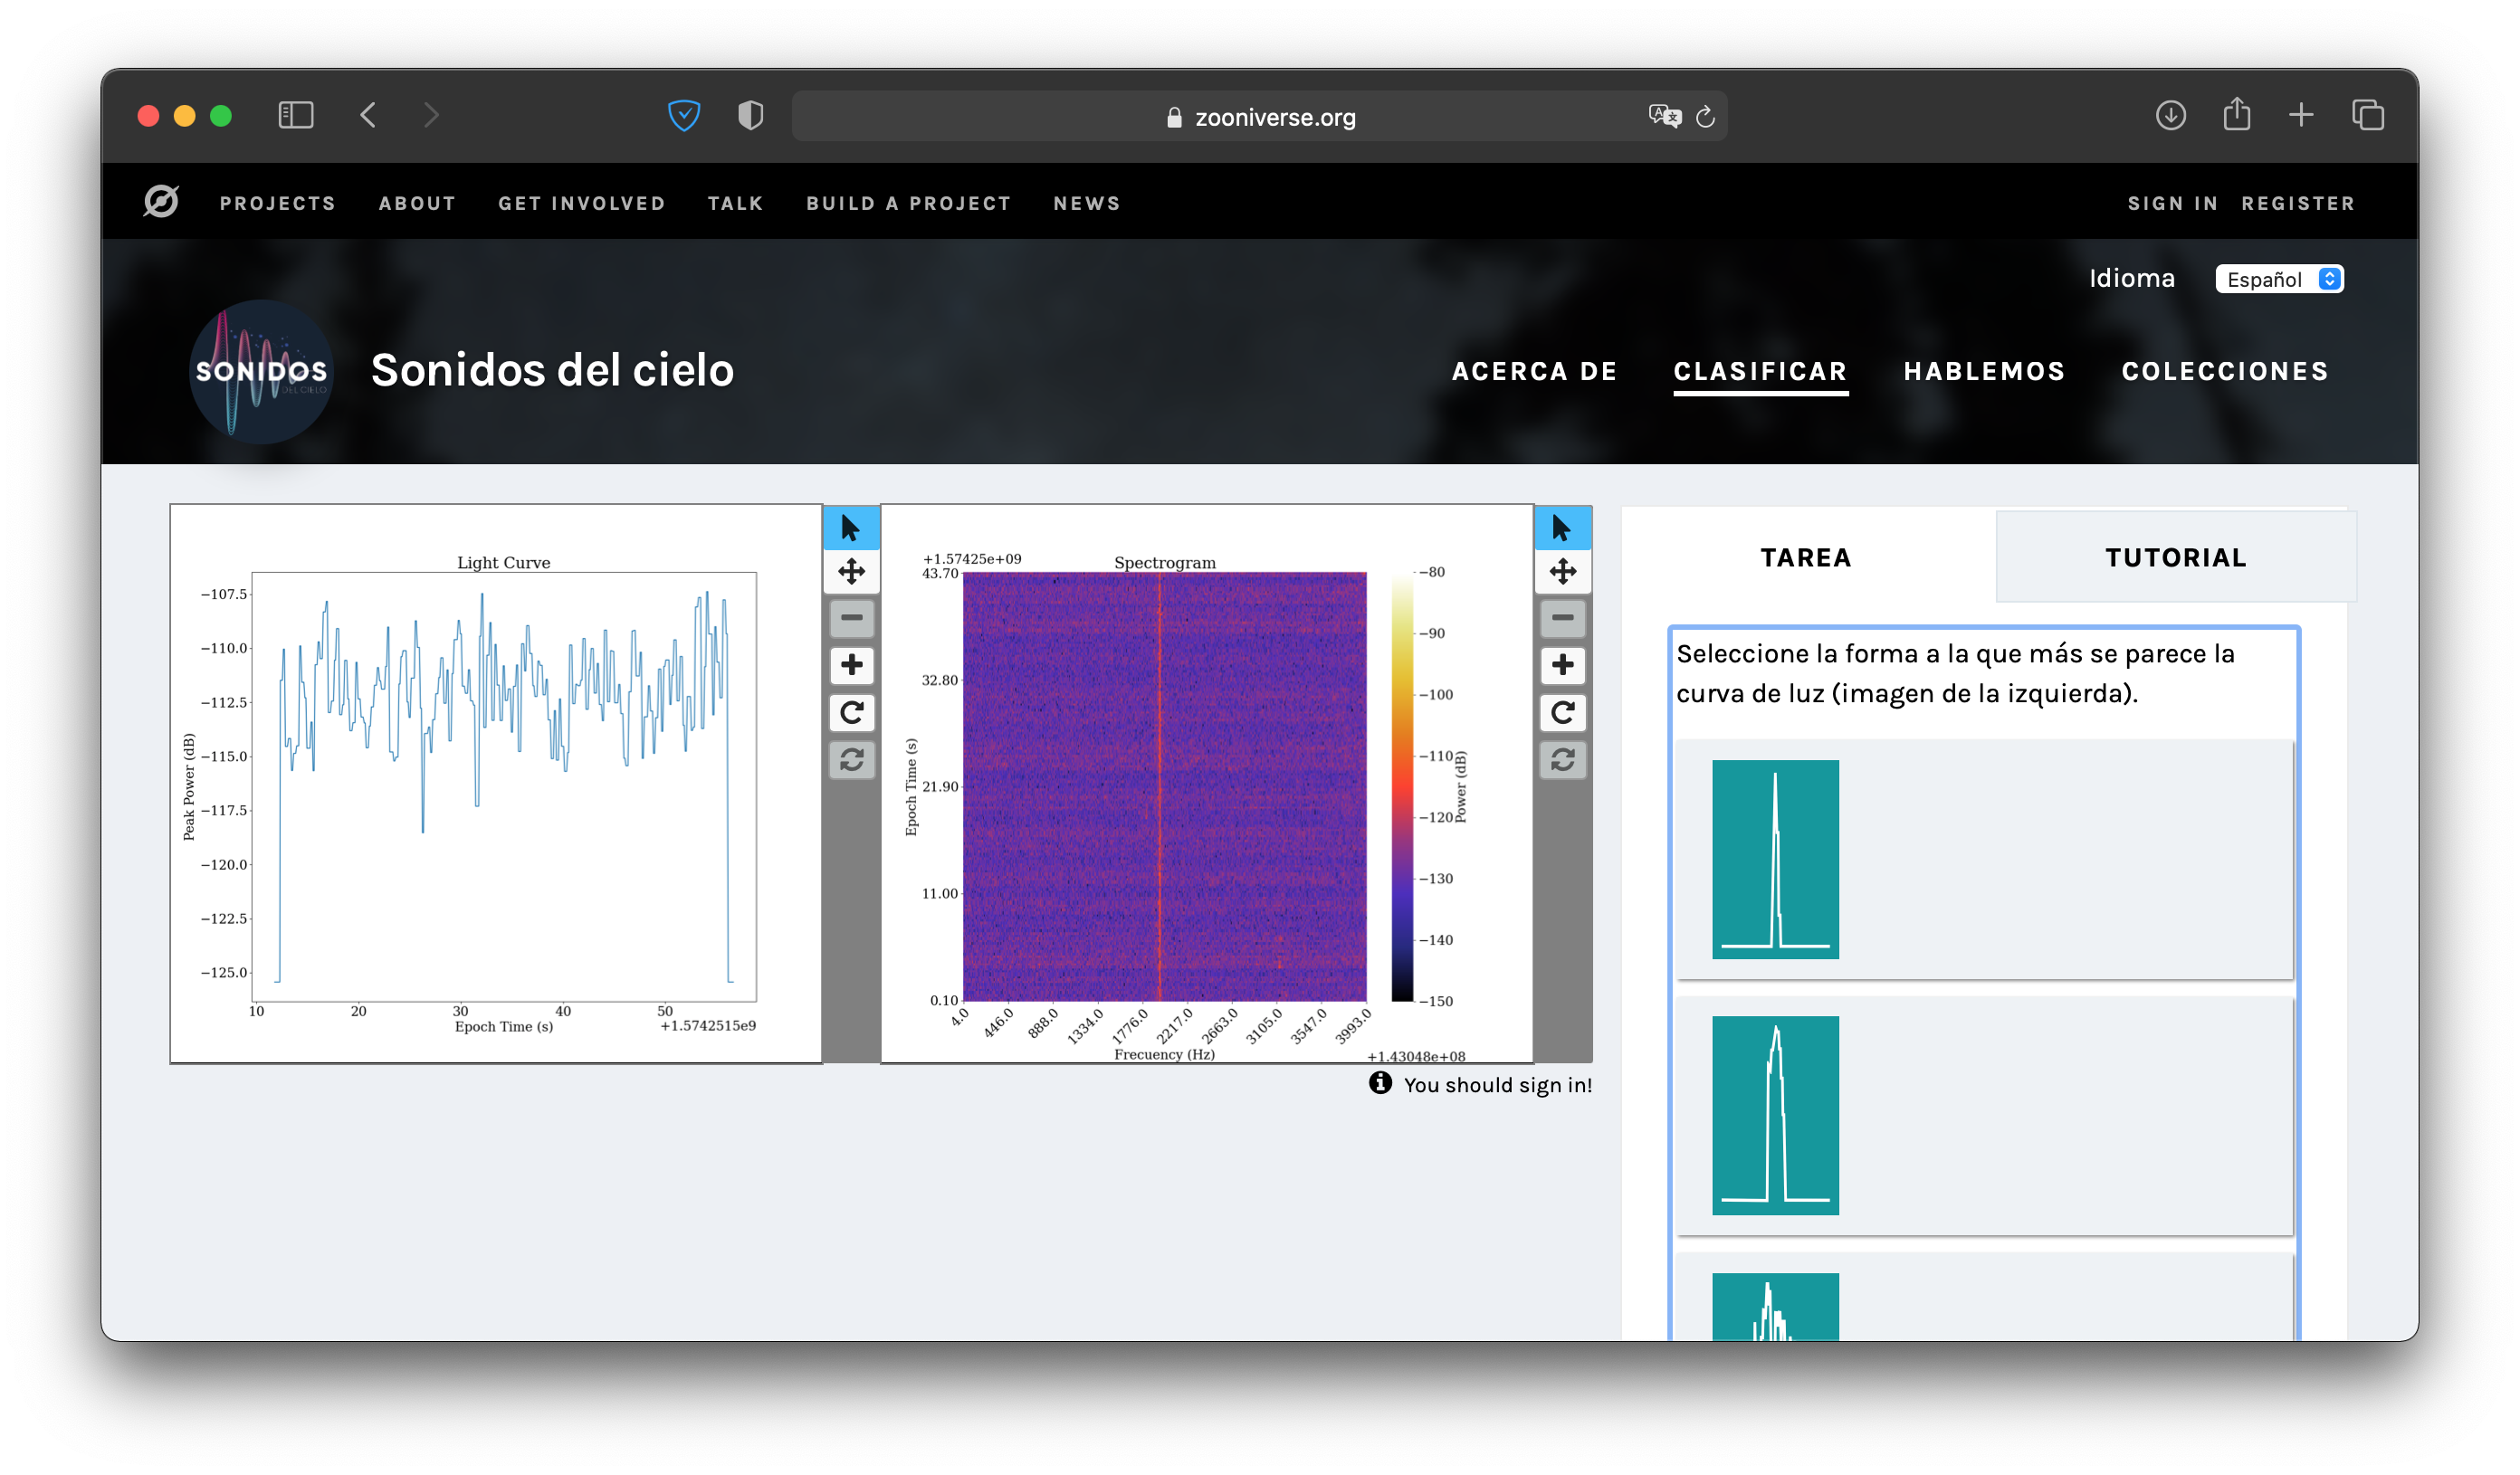
\includegraphics[width=\textwidth]{include/figuras/Zooniverse.png}
    \caption{Clasificación en el portal Zooniverse}
    \label{fig:web_zooniverse}
\end{figure}

La idea del proyecto es realizar una herramienta paralela a este servicio a través de la cual los ciudadanos puedan contribuir con la clasificación de cuerpos celestes, y que sea utilizable tanto por adultos como por niños y gente con algún tipo de discapacidad visual.

El proyecto es responsabilidad de el equipo de investigadores y estudiantes del Citizen Science Lab de la Universidad Politécnica de Madrid en colaboración con el Instituto Astrofísico de Canarias, el Grupo Docente de Astronomía Kepler y la Agrupación Astronómica Madrid Sur, representadas en la figura \ref{fig:empresas} y tiene como objetivo la detección y catalogación estos meteoroides.

\begin{figure} [h]
    \centering
    
\includegraphics[width=\textwidth]{include/figuras/Empresas_proyecto.png}
    \caption{Empresas impulsoras del proyecto}
    \label{fig:empresas}
\end{figure}

En la actualidad los meteoros son conocidos por el público general debido a las lluvias de estrellas, las más conocidas son las Perseídas que de producen de manera anual entre los meses de julio y agosto; y las Gemínidas que provienen de un asteroide conocido como Faetón y se pueden observar en el mes de diciembre. La ambición de este proyecto es despertar el interés en los ciudadanos y realizar una tarea de divulgación desde un punto de vista científico. 
Para poder detectar los meteoros se cuenta actualmente con una infraestructura de dos estaciones de radiodetección situadas en Fuenlabrada (Madrid) y Fregenal de la Sierra (Badajoz) construidas por miembros aficionados de la Agrupación Astronómica de Madrid Sur y del Grupo Docente de Astronomía Kepler \cite{kepler}, estas dos estaciones monitorizan la señal del radar GRAVES \cite{graves} ubicado en Dijón (Francia) que emite a 143.050 MHz mediante varias antenas de tipo Yagi, un receptor SDR \cite{ulversoy2010software}, se puede ver el funcionamiento del radar en la figura\ref{fig:radar}. A través del programa de código abierto Echoes \cite{echoes} es posible generar una curva de luz, un espectrograma de esta detección y posteriormente generar a partir de ellas el sonido del meteoroide. 

\begin{figure} [h]
    \centering
    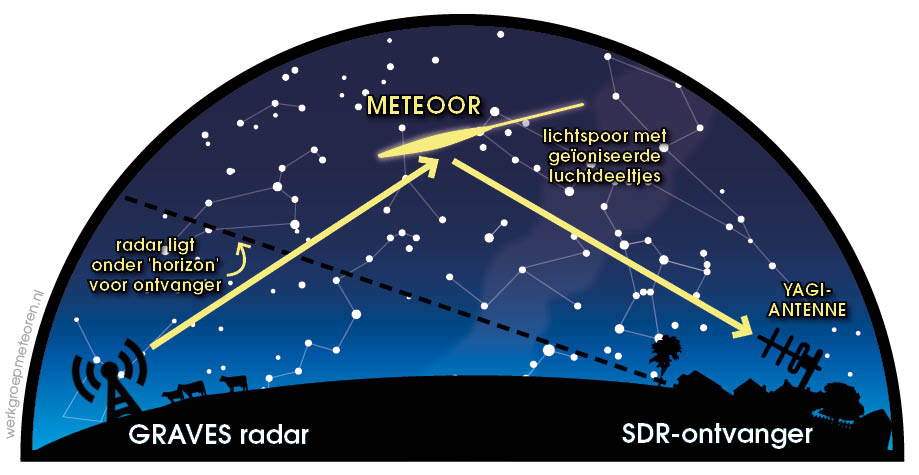
\includegraphics[scale=0.35]{include/figuras/Radar.jpg}
    \caption{Funcionamiento del radar GRAVES}
    \label{fig:radar}
\end{figure}

\vspace{0.5cm}

%En el contexto del proyecto se quiere acercar la astronomía a los ciudadanos, ya sean adultos o niños y además hacerla accesible para personas con discapacidad visual. Como parte del proyecto se creará un asistente automatizado apoyado en la inteligencia artificial mediante el cual guiará a los usuarios para ayudarlos a realizar la clasificación de los cuerpos celestes, ya sea a través de escritura o por voz.
%Como resultado del proyecto se pretende conseguir una clasificación de los meteoros y contrastarla con las publicadas en artículos científicos.


\section{Objetivos}

Puesto que el proyecto ha recibido financiación ha sido necesario realizar la contratación de un desarrollador que se una al equipo a colaborar con el desarrollo de las distintas herramientas. Esto ha provocado que se reajusten las tareas a realizar por los miembros del equipo y  los requisitos del Trabajo de Fin de Grado puesto que era necesario desarrollar las herramientas que fuesen la base del proyecto. A continuación se listan los objetivos del proyecto:

%El objetivo principal de este trabajo de fin de grado es la construcción de un asistente virtual o chatbot que sea capaz de comunicarse con un usuario de forma autónoma. También se va a desarrollar todo el backend sobre el que se sostiene el proyecto Sonidos del Cielo del departamento de ciencia ciudadana de la Universidad Politécnica de Madrid.

%Los objetivos del proyecto son los siguientes:
%Mejora de la interfaz conversacional de un chatbot.
%Integración de módulos de reconocimiento y sintetizador de voz.
%Desarrollo de una interfaz web del experimento de clasificación de meteoros para público infantil.
%Módulo para analizar los resultados obtenidos. 
%Desarrollo de una guía de usuario.

\begin{itemize}
    \item Diseño y desarrollo de la arquitectura de la base de datos del proyecto.
    \item Diseño y desarrollo de la API del proyecto.
    \item Integración de la API con la base de datos del proyecto.
    \item Creación de scripts para la inserción automática de nuevas detecciones de meteoros.
    \item Creación de una versión preliminar del chatbot para probar las funcionalidades de la API.
\end{itemize}

\section{Estructura del documento}

\begin{itemize}
\item Capítulo 2: Este capítulo es el estado del arte sobre las tecnologías en las que está basado el trabajo de fin de grado. 
\item Capítulo 3: En este capítulo se detallan las herramientas utilizadas y el desarrollo del proyecto.
\item Capítulo 4: En este capítulo se especifican los resultados del trabajo y las posibles mejoras a implementar.
\item Bibliografía: publicaciones utilizadas en el estudio y desarrollo del trabajo.
\item Anexos (opcional)
\end{itemize}
